\chapter{Конструкторский часть}

В данном разделе представлены схемы алгоритмов DBSCAN и конвейера.

\section{Разработка алгоритмов}

\subsection{Разработка простого DBSCAN}
 
На рисунке \ref{fig:alg} приведена схема плотностного алгоритма DBSCAN.


\begin{figure}[ht!]
	\centering
	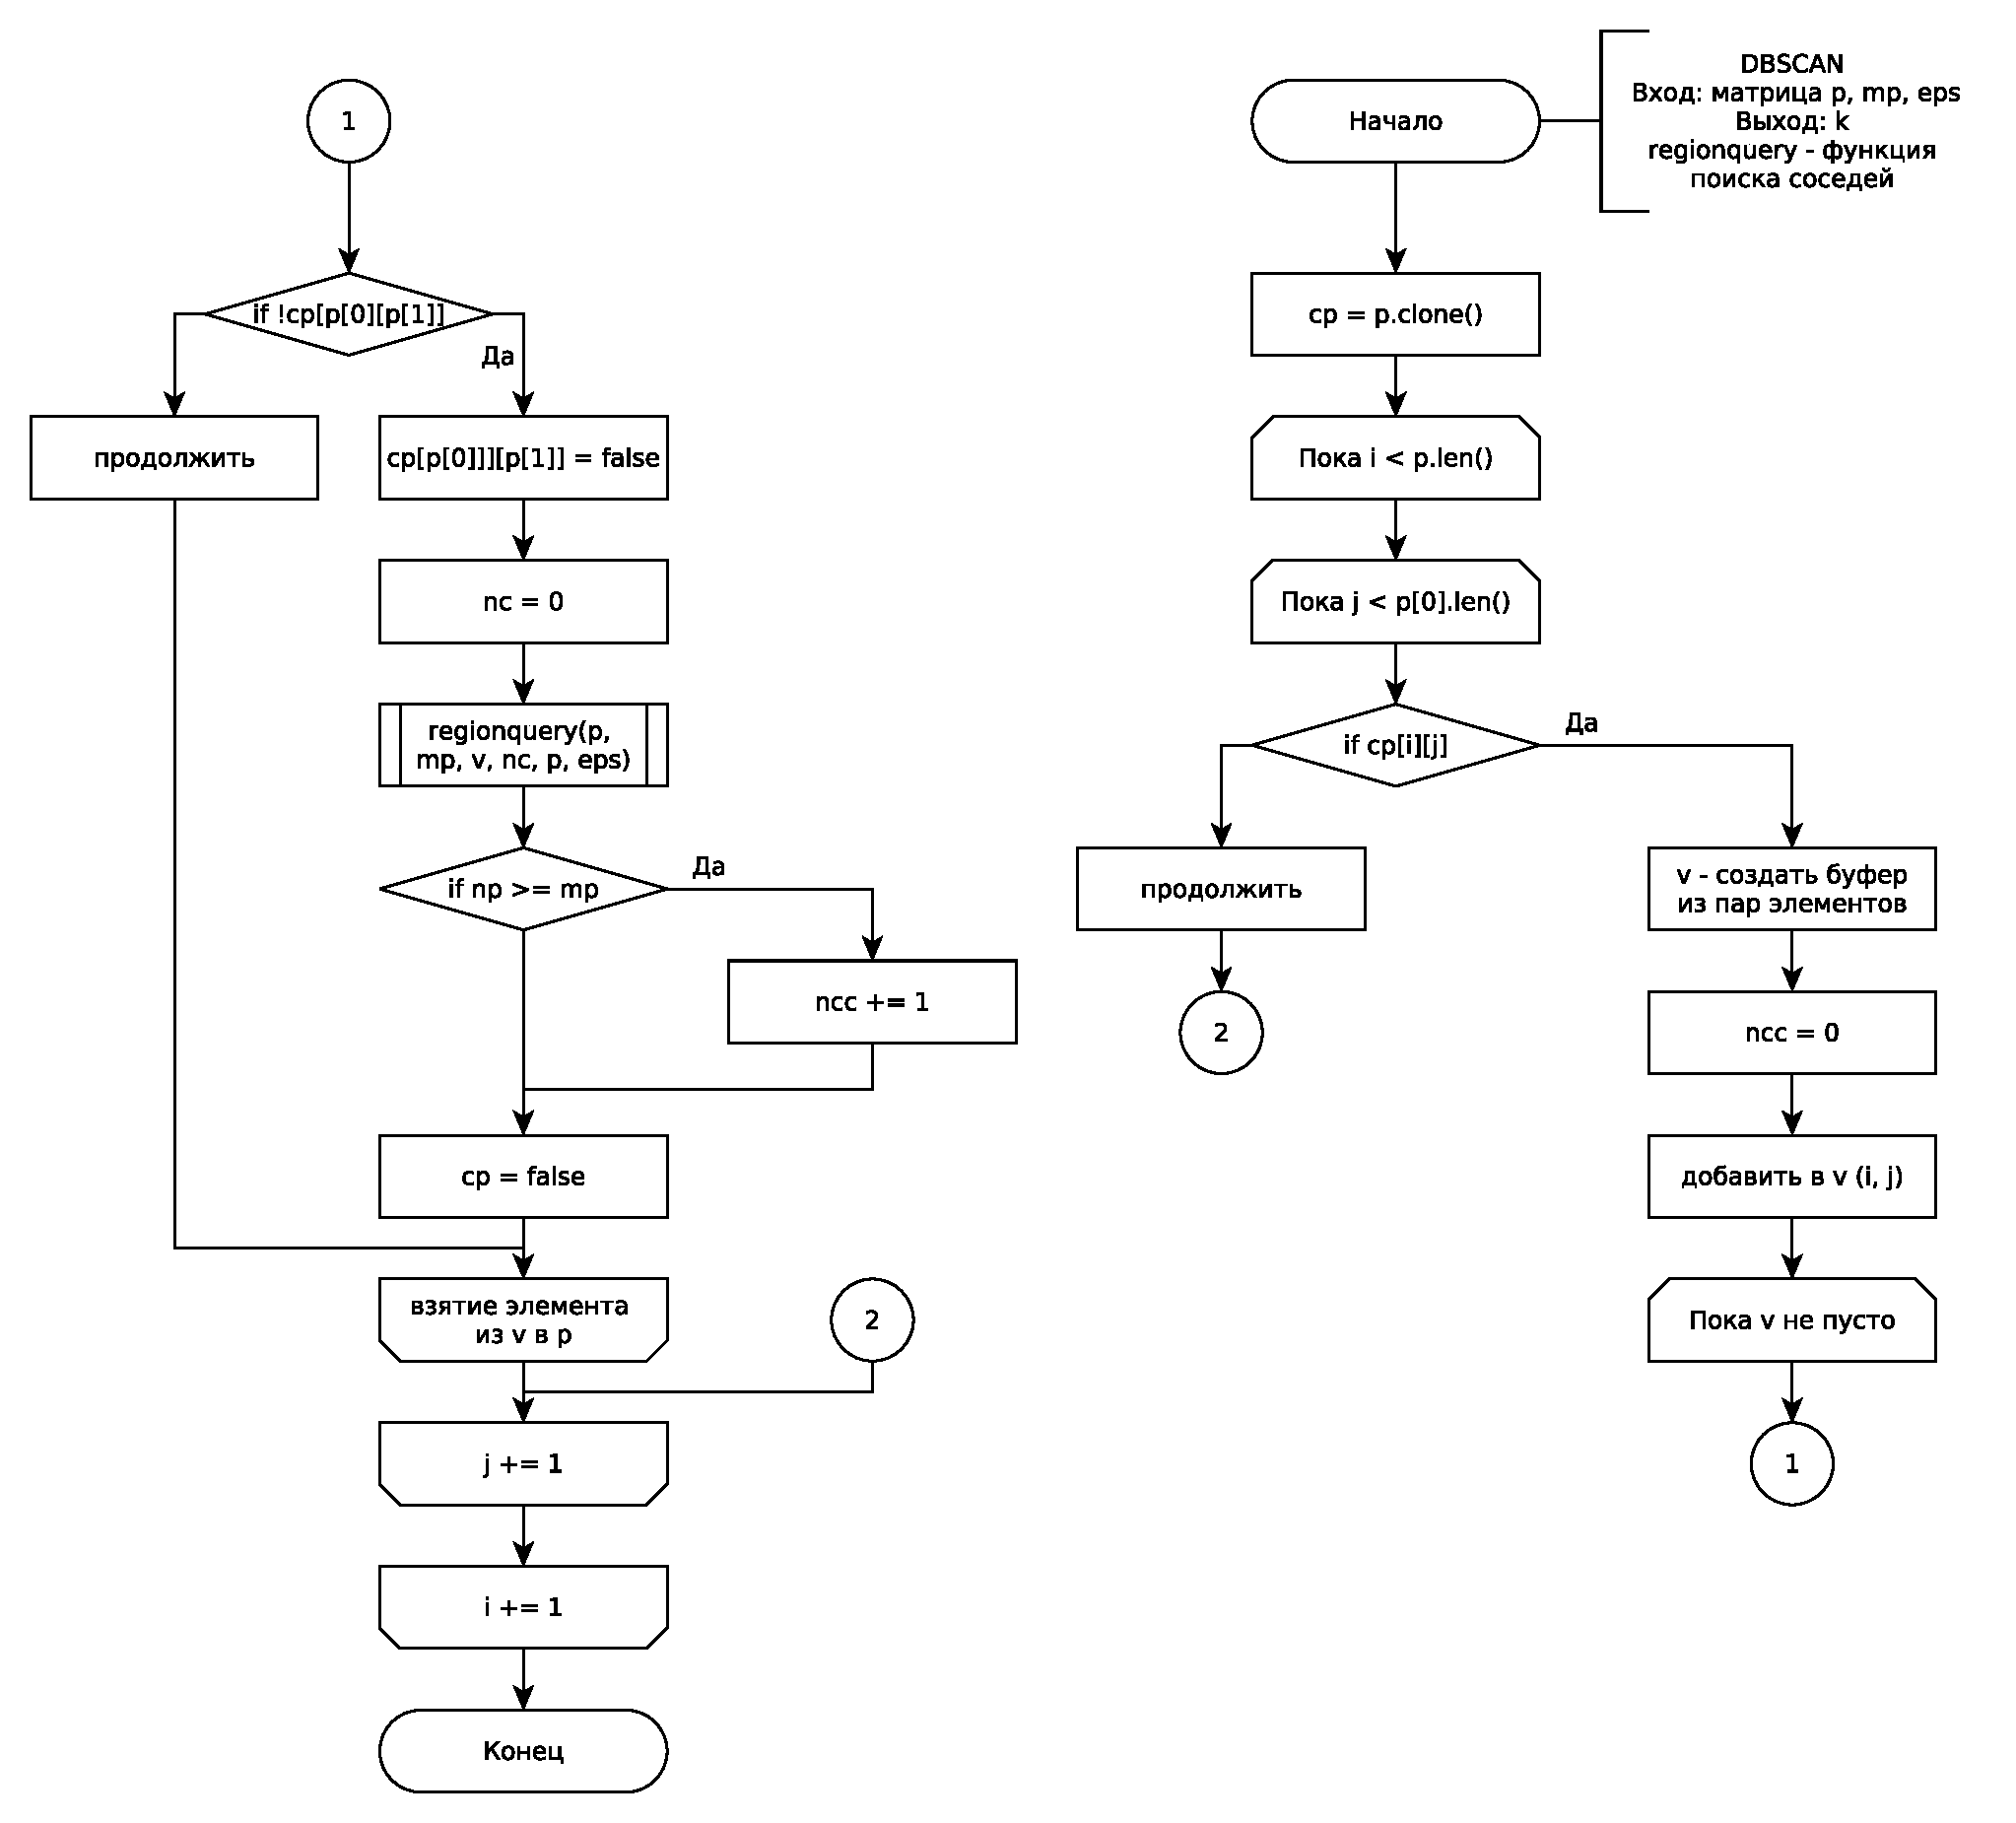
\includegraphics[width=1\linewidth]{assets/graphs/dbscan.pdf}
	\caption{Схема плотностного алгоритма DBSCAN}
	\label{fig:alg}
\end{figure}

На рисунке \ref{fig:alg2} приведена схема функции поиска ближайшей соседний точки в кластере.

\begin{figure}[ht!]
	\centering
	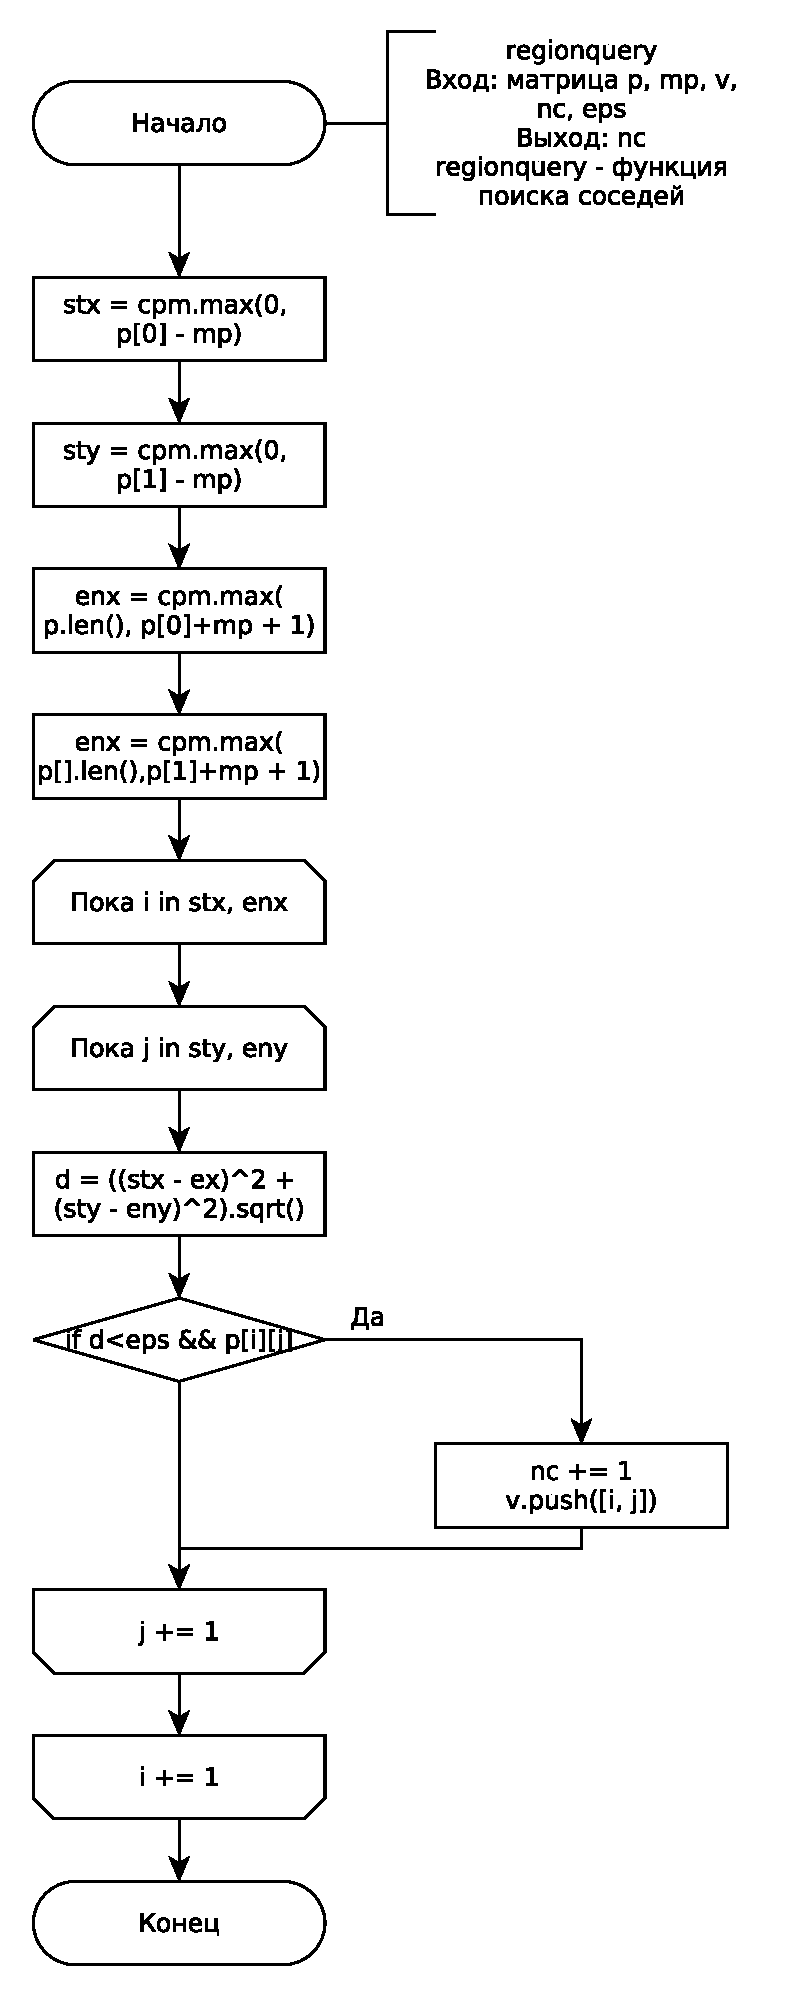
\includegraphics[width=0.5\linewidth]{assets/graphs/regionquery.pdf}
	\caption{Схема функции regionquery}
	\label{fig:alg2}
\end{figure}

\subsection{Разработка конвейерных вычислений}

На рисунке \ref{fig:alg-p} приведена схема конвейерной линии.

\begin{figure}[ht!]
	\centering
	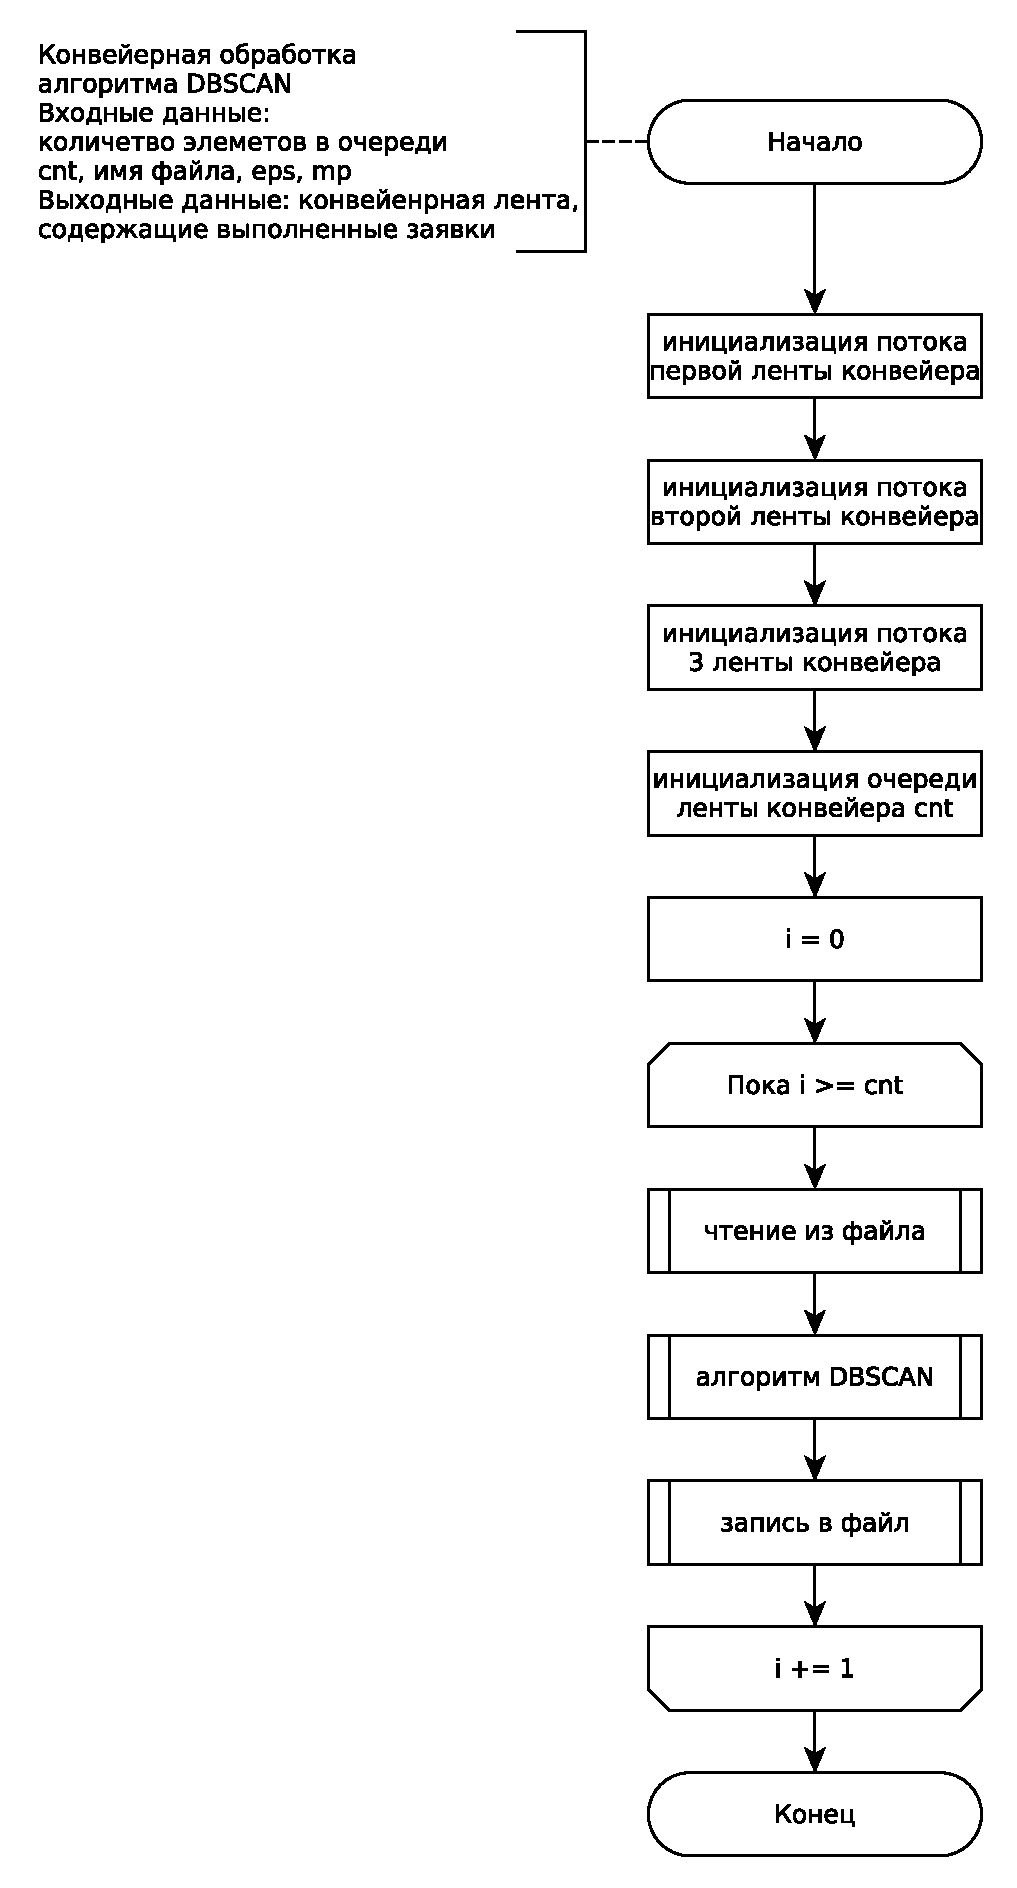
\includegraphics[width=0.7\linewidth]{assets/graphs/pipeline.pdf}
	\caption{Схема алгоритма параллельного DBSCAN}
	\label{fig:alg-p}
\end{figure}


\section*{Вывод}

Были разработаны схемы алгоритмов, необходимых для решения задачи.